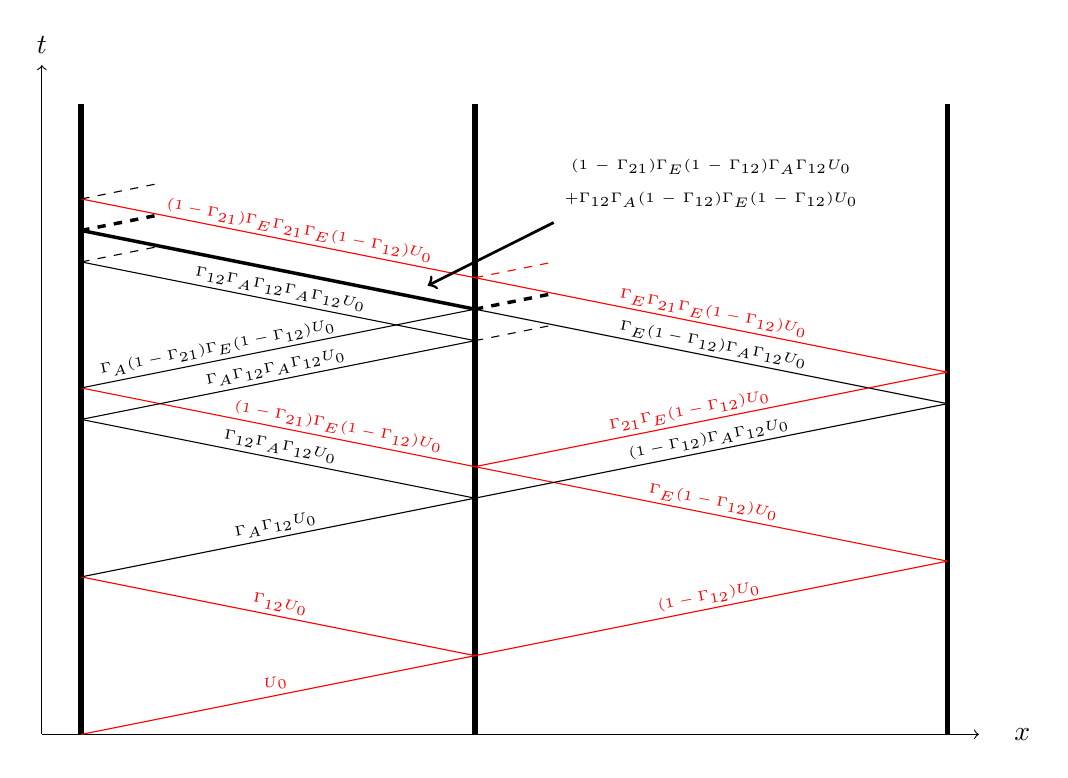
\begin{tikzpicture}
	\draw[line width=2pt] (0,0) -- (0,8);
	\draw[line width=2pt] (11,0) -- (11,8);
	\draw[line width=2pt] (5,0) -- (5,8);
	\draw[->] (-0.5,0) -- node [yshift = 4.5cm]{$t$} (-0.5,8.5);
	\draw[->] (-0.5,0) -- node [xshift = 6.5cm]{$x$} (11.4,0);
	
	% Strahl1
	\draw[color=red] (0,0) -- node [rotate=11,yshift=0.15cm]{\tiny$U_0$} (5,1);
	\draw[color=red] (5,1) -- node [rotate=11,yshift=0.15cm]{\tiny$(1-\Gamma_{12})U_0$} (11,1/5*11);
	\draw[color=red] (11,1/5*11) -- node [rotate=-11,yshift=0.15cm]{\tiny$\Gamma_E(1-\Gamma_{12})U_0$} (5,1/5*11+1/5*6);
	\draw[color=red] (5,1/5*11+1/5*6) -- node [rotate=-11,yshift=0.15cm,xshift=0.75cm]{\tiny$(1-\Gamma_{21})\Gamma_E(1-\Gamma_{12})U_0$} (0,1/5*11*2);
	\draw (0,1/5*11*2) -- node [rotate=11,yshift=0.15cm,xshift=-0.75cm]{\tiny$\Gamma_A(1-\Gamma_{21})\Gamma_E(1-\Gamma_{12})U_0$} (5,1/5*11*2 + 1);
	\draw[dashed,line width=1.25pt] (5,1/5*11*2 + 1) -- (6,1/5*11*2+1+1/5);

	% Strahl2
	\draw[color=red] (5,1) -- node [rotate=-11,yshift=0.15cm]{\tiny$\Gamma_{12}U_0$} (0,2);
	\draw (0,2) -- node [rotate=11,yshift=0.15cm]{\tiny$\Gamma_A\Gamma_{12}U_0$} (5,3);
	\draw (5,3) -- node [rotate=11,yshift=0.15cm]{\tiny$(1-\Gamma_{12})\Gamma_A\Gamma_{12}U_0$} (11,1/5*11+2);
	\draw (11,1/5*11+2) -- node [rotate=-11,yshift=0.15cm]{\tiny$\Gamma_E(1-\Gamma_{12})\Gamma_A\Gamma_{12}U_0$} (5,1/5*11+1/5*6+2);
	\draw[line width=1.25pt] (5,1/5*11+1/5*6+2) -- (0,1/5*11+1/5*6+2+1);
	\draw[dashed,line width=1.25pt] (0,1/5*11*2+2) -- (1,1/5*11*2+2+1/5);
	
	%Strahl3
	\draw (5,3) -- node [rotate=-11,yshift=0.15cm]{\tiny$\Gamma_{12}\Gamma_A\Gamma_{12}U_0$} (0,4);
	\draw (0,4) -- node [rotate=11,yshift=0.15cm]{\tiny$\Gamma_A\Gamma_{12}\Gamma_A\Gamma_{12}U_0$} (5, 1+4);
	\draw[dashed] (5, 5) -- (6, 1/5+5);
	
	%Strahl4
	\draw (5,5) -- node [rotate=-11,yshift=0.15cm]{\tiny$\Gamma_{12}\Gamma_A\Gamma_{12}\Gamma_A\Gamma_{12}U_0$} (0,6);
	\draw[dashed] (0,6) -- (1,1/5+6);

	%Strahl5
	\draw[color=red] (5,1/5*11*2-1) -- node [rotate=11,yshift=0.15cm,xshift=-0.25cm]{\tiny$\Gamma_{21}\Gamma_E(1-\Gamma_{12})U_0$} (11,1/5*11*2-1+1/5*6);
	\draw[color=red] (11,1/5*11*2-1+1/5*6) -- node [rotate=-11,yshift=0.15cm]{\tiny$\Gamma_E\Gamma_{21}\Gamma_E(1-\Gamma_{12})U_0$} (5,1/5*11*2-1+1/5*6*2) -- node [rotate=-11,yshift=0.15cm,xshift=0.25cm]{\tiny$(1-\Gamma_{21})\Gamma_E\Gamma_{21}\Gamma_E(1-\Gamma_{12})U_0$} (0,1/5*11*2-1+1/5*6+1/5*11);
	\draw[dashed] (0,1/5*11*2-1+1/5*6+1/5*11) -- (1,1/5*11*2-1+1/5*6+1/5*11 + 1/5);
	
	%Strahl6
	\draw[dashed,color=red] (5,1/5*11*2-1+1/5*6*2) -- (6,1/5*11*2-1+1/5*6*2+1/5);
	
	\draw[<-,line width=1pt] (4.4,1/5*11+1/5*6+2+1/5+0.1) -- (6,6.5);
	\draw (8,7) node[text width=5cm,align=center]{\tiny$(1-\Gamma_{21})\Gamma_E(1-\Gamma_{12})\Gamma_A\Gamma_{12}U_0$ \\ $+ \Gamma_{12}\Gamma_A(1-\Gamma_{12})\Gamma_E(1-\Gamma_{12})U_0$} (11,7);
\end{tikzpicture} \\